%----------------------------------------------------------------------------
\chapter{Validáció}
\label{chp:validation}
%----------------------------------------------------------------------------
\begin{itemize}
  \item a két alfejezet rövid tartalma jön ide
\end{itemize}

%----------------------------------------------------------------------------
\section{Tesztelés}
%----------------------------------------------------------------------------
\begin{itemize}
  \item a készített alkalmazás egy adott bemenettel történő futását kísérjük nyomon:
  \item tesztkörnyezet bemutatása, milyen szempontok alapján lett összeállítva
  \item program futásának végigkövetése (sok screenshottal)
  \item értékelés
\end{itemize}

%----------------------------------------------------------------------------
\section{Teljesítményelemzés}
%----------------------------------------------------------------------------
A programom teljesítményének elemzéséhez a következő méréseket végeztem el:

\begin{itemize}
  \item 1,2,4 és 8 GiB méretű fájlok terítése 10 ill. 25 gépre
  \item 4 GiB méretű fájl terítése 25 gépre háromször, különbőző seed választásával
  \item Hibatűrési tesztek a terítés elején hiányző, ill. aközben kieső gépekkel.
\end{itemize}

Továbbá, hogy legyen összehasonlítási alap  az eredeti Chaincast alapú terítést is lefuttattam 25 gépre 1,2,4 és 8 GiB méretű fájlokkal.
A mérési eredmények az alkalmazásom futásakor keletkező logfájlból származnak, Chaincast esetében pedig a Jenkins webes felületén a terítéshez tartozó build ``build output'' részből.

%
\subsection{Chaincast és Torrent alapú terítés idejének összehasonlítása}
%

Nem a gyorsabb fájlterítés megvalósítása volt a programom egyik célja, de attól még érdemes lehet összehasonlítanunk a két módszer sebességét, hiszen mindegy mennyit nyerünk a robusztusságon , ha használhatatlanul lassabb lesz az alkalmazás a mostaninál. Az~\ref{fig:chaincasttorrrentcomparison}-es~ábrán láthatjuk a különbőző méretű fájlok terítésének az idejét. Előtte visztont érdemes részletesebben megnézni, hogy ez az idő konkrétan mit (nem) tartalmaz:

\begin{itemize}
  \item Egyik megoldásnál sem tartalmazza a terítés ideje a terítendő fájlok létrehozását, és a központi gépre másolását (ami egyik esetben egy hálózati meghajtó, másik esetben a torrent-es terítés seed-je)
  \item Torrent-es terítésnél az időt a fájl hash-elése előtt, illetve után kezdjük mérni, Chaincast-nál a webes felületen a terítés indításától
\end{itemize}

Az előbbi állítások a későbbi mérésekre is igazak lesznek.

\begin{figure}[ht]
\centering
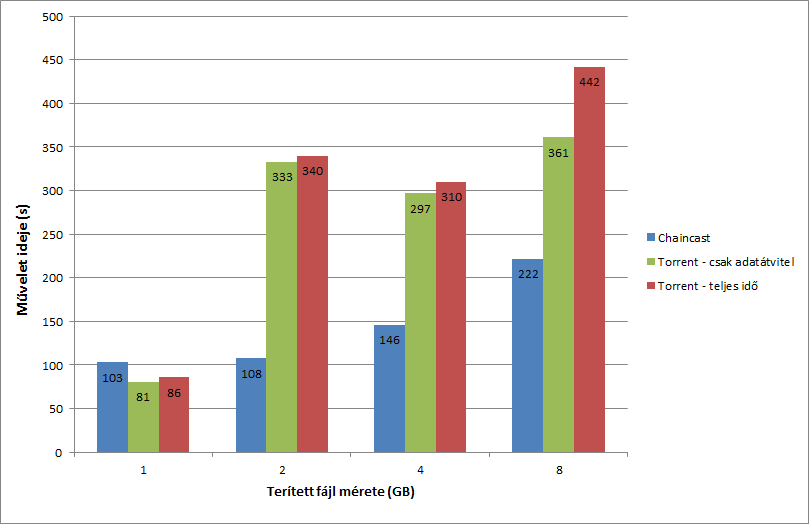
\includegraphics[width=150mm, keepaspectratio]{figures/Perf_chaincast_torrent_comparison.png}
\caption{Chaincast és Torrent alapú terítés idejének összehasonlítása}
\label{fig:chaincasttorrrentcomparison}
\end{figure}


Ide írom, hogy milyen következtetést kellene levonni az ábráról.
meglepó, hogy 2 g milyen lasssú, kis fájlnál nem nagyon van kül
nagyobb fájloknál kb 2x lassabb terítés , ez elfogadható, főleg hogy azt tapasztalam, hogy átlagosan 2 prbóálkozás kell egy sikeres chaincasthoz, ami ha a végém szakadna meg akkor hasonló időt vesz igénybe
esetleg még a hashelés által okozott overhead a fájl méretével egyenesen arányosan nő


%
\subsection{Skálázódás - Torrentes terítés 10 és 25 gépere}
%

A Torrent-től, mint P2P alapú fájlmegosztó protokolltól azt várjuk, hogy letöltők számával minimum nem fordítottan arányos a terítés idje, vagyis több résztvevő esetén sem tart több ideig a fájlátvitel. Most 10 és 25 gépre történő térítés esetén hasonlítjuk össze teljesítménymutatókat a övetkező táblázat segítségével:

\begin{center}
	\begin{tabular}{ |c|>{\centering\arraybackslash}m{2.5cm}|>{\centering\arraybackslash}m{2.5cm}|>{\centering\arraybackslash}m{2.5cm}|>{\centering\arraybackslash}m{2.5cm}| }
		\hline
		\multirow{2}{*}{Fájlméret}&\multicolumn{2}{|c|}{Terítés - teljes idő}&\multicolumn{2}{|c|}{Terítés - csak az adatátvitel} \\
		& 10 gépre & 25 gépre & 10 gépre & 25 gépre \\
		\hline
		1 GiB & 85 s & 86 s & 80 s & 81 s \\
		\hline
		2 GiB & 178 s & 340 s & 167 s & 333 s \\
		\hline
		4 GiB & 293 s & 310 s & 270 s & 297 s \\
		\hline
		8 GiB & 563 s & 442 s & 516 s & 361 s \\
		\hline
	\end{tabular}
\end{center}

[a szegélyeket hogyan lehetne szépre megcsinálni?]\\

Ennek az elemzése\ldots
%
\subsection{Terítés ideje különbőző seed-ek választása esetén}
%

Érdemes lehet megnézni, hogy különbőző seed gépek választása hogyan befolyásolja a terítés idejét, ezért lefuttattam a 4 GiB-es fájl terítését 25 gépre háromszor, különbőző seed-eket választva. Az eredményt az~\ref{fig:differentseedscomparison}-es~ábra szemlélteti. 

\begin{figure}[ht]
\centering
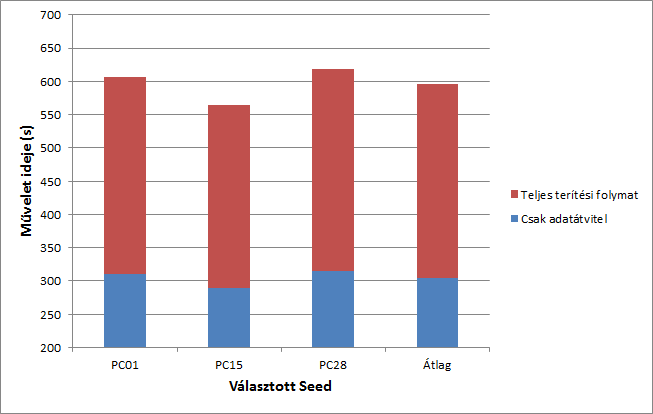
\includegraphics[width=120mm, keepaspectratio]{figures/Perf_different_seeds.png}
\caption{Terítés ideje különbőző seed-ek választása esetén}
\label{fig:differentseedscomparison}
\end{figure}

Nagonyrövid tanulság levonása.

%
\subsection{P2P alapú fájlterítés - hibatűrése}
%

%
\subsection{P2P alapú fájlterítés - szűk keresztmetszetek keresése}
%

\begin{figure}[ht]
\centering
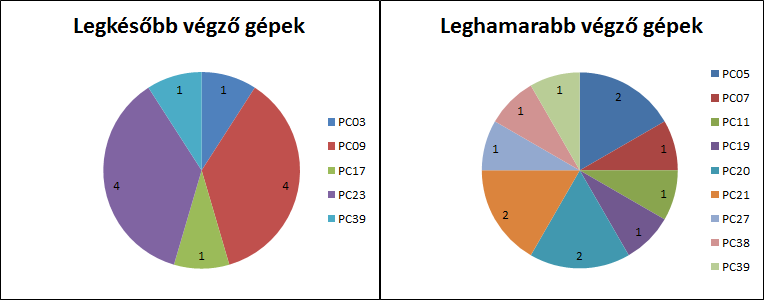
\includegraphics[width=150mm, keepaspectratio]{figures/Perf_computers.png}
\caption{Letöltést leghamarabb/legkésőbb befejező gépek}
\label{fig:computerdownloadspeeds}
\end{figure}

%
\subsection{P2P alapú fájlterítés - letöltési sebességek}
%

